\documentclass[xcolor=svgnames, aspectratio=169]{beamer}
\usepackage{pgfpages}
\setbeameroption{
  hide notes
  % show notes
  % show notes on second screen=right  % requires pgfpages
  % show only notes
}

\definecolor{mygreen}{rgb}{.125,.5,.25}

\setbeamertemplate{note page}{
  \vspace{.5cm}\hspace{.8\textwidth}
  \vspace{-2.7cm}
  \fbox{\insertslideintonotes{.2}}
  \pagecolor{white}
  \LARGE
  \begin{tikzpicture}[remember picture,overlay]
    \node [color=mygreen, opacity=0.8, xshift=-.3cm, yshift=-1.9cm, rotate=90] (current page.north west) {\bfseries N O T E S};
  \end{tikzpicture}
  \footnotesize
  \insertnote
}

% --- THEME ---
\usetheme[progressbar=frametitle]{metropolis}

\useoutertheme{metropolis}
\useinnertheme{metropolis}
\usefonttheme{metropolis}
\usecolortheme{spruce}  % spruce, metropolis, dove, crane, beaver, seagull
\setbeamercolor{background canvas}{bg=white}
\usecolortheme[named=mygreen]{structure}
\usefonttheme[onlymath]{serif}

% --- HACKS ---
% Hide numbers on standout slides.
\setbeamertemplate{frame numbering}{
    \ifbool{metropolis@standout}{}{
        \insertframenumber
    }
}
\setbeamertemplate{frame numbering}[counter]  % none, counter, fraction

% Avoid font-warning with itemize bullets.
\renewcommand\textbullet{\ensuremath{\bullet}}

% --- PACKAGES ---
\usepackage[UKenglish]{babel}
\usepackage[utf8]{inputenc}
\usepackage{lmodern}
\usepackage[T1]{fontenc}

% \usepackage{appendixnumberbeamer}
\usepackage{upquote}
\usetikzlibrary{positioning}
% \usepackage{minted}
\usepackage{multicol}
\usepackage{xspace}
\usepackage{booktabs}
\usepackage{siunitx}

% --- SETTINGS ---
\graphicspath{{./figures/}}
\setlength{\fboxsep}{0pt}

% --- OWN COMMANDS ---
\newcommand{\bdra}{\ensuremath{\boldsymbol \Rightarrow }~}
\newcommand{\bdla}{\ensuremath{\boldsymbol \Leftarrow }~}
\newcommand{\dra}{\ensuremath{\Rightarrow }~}
\newcommand{\dla}{\ensuremath{\Leftarrow }~}
\newcommand{\mr}[1]{\mathrm{#1}}
\newcommand{\emg}[2]{\texttt{emg#1#2}\xspace}
\newcommand{\empymod}{\texttt{empymod}\xspace}
\newcommand{\simpeg}{\texttt{SimPEG}\xspace}
\newcommand{\discretize}{\texttt{discretize}\xspace}
\newcommand{\custem}{\texttt{custEM}\xspace}
\newcommand{\petgem}{\texttt{PETGEM}\xspace}
\newcommand{\ohmm}{\ensuremath{\Omega\,}\text{m}\xspace}
\newcommand{\rmk}[1]{{\color{red}\bfseries #1}}
\newcommand{\maybe}[1]{{\color{gray} #1}}
\newcommand{\todo}{{\color{red}\texttt{TODO:}}\xspace}

% --- SLIDES ---
\begin{document}
\metroset{block=fill}  % Fills the block-environment

\begin{frame}[c]%
  {Open-Source Landscape for Three-Dimensional CSEM Modeling}
  \vspace{.3cm}
  \begin{columns}[c]
    \column{.3\textwidth}
      \centering
      
\includegraphics[width=2.0cm]{Logo-emg3d}\\[.5cm]
      
\includegraphics[width=2.0cm]{Logo-custEM}\\[.5cm]
      
\includegraphics[width=2.2cm]{Logo-PETGEM}\\[.5cm]
      
\includegraphics[width=3.0cm]{Logo-SimPEG2}
    %
    \column{.7\textwidth}
      ~\\\vspace{.4cm}
      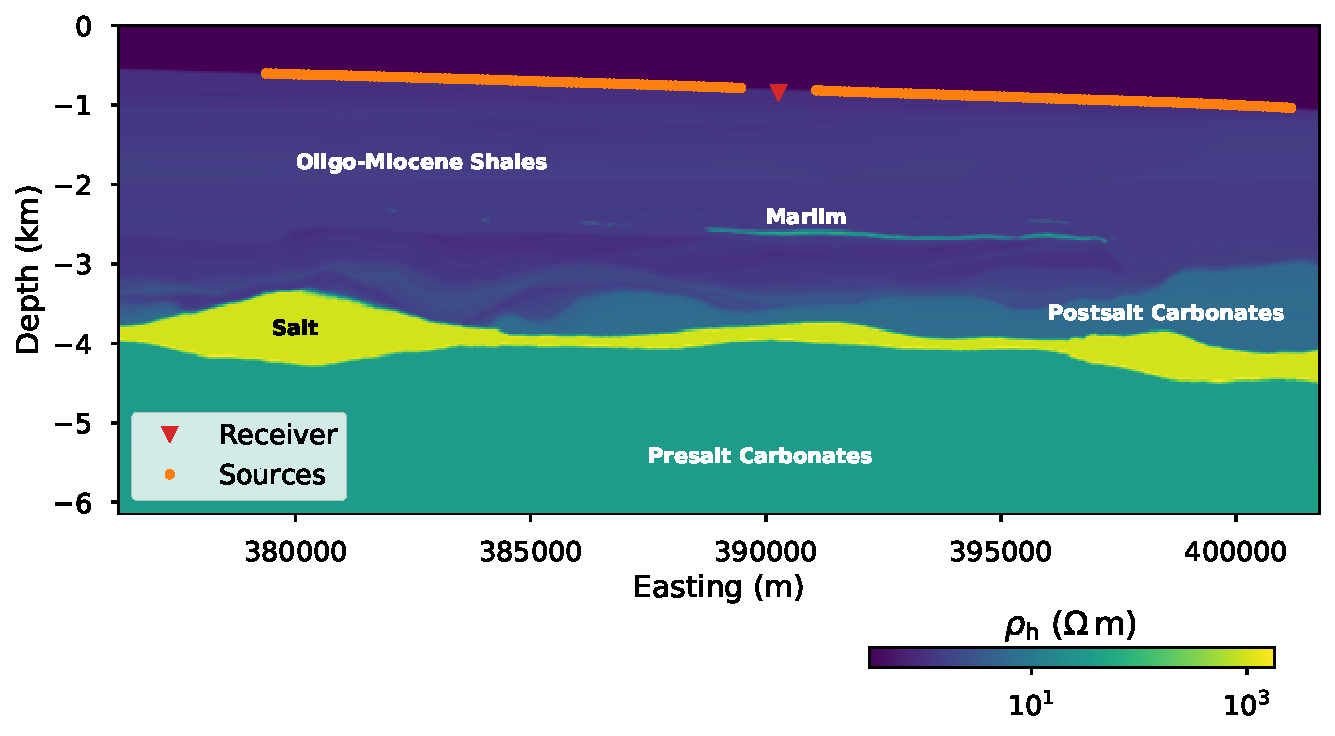
\includegraphics[width=.9\textwidth]{model-marlim}\\[.5cm]
      \begin{tikzpicture}[remember picture,overlay]
        \node [color=white, xshift=8cm, yshift=5.5cm] (current page.south west) {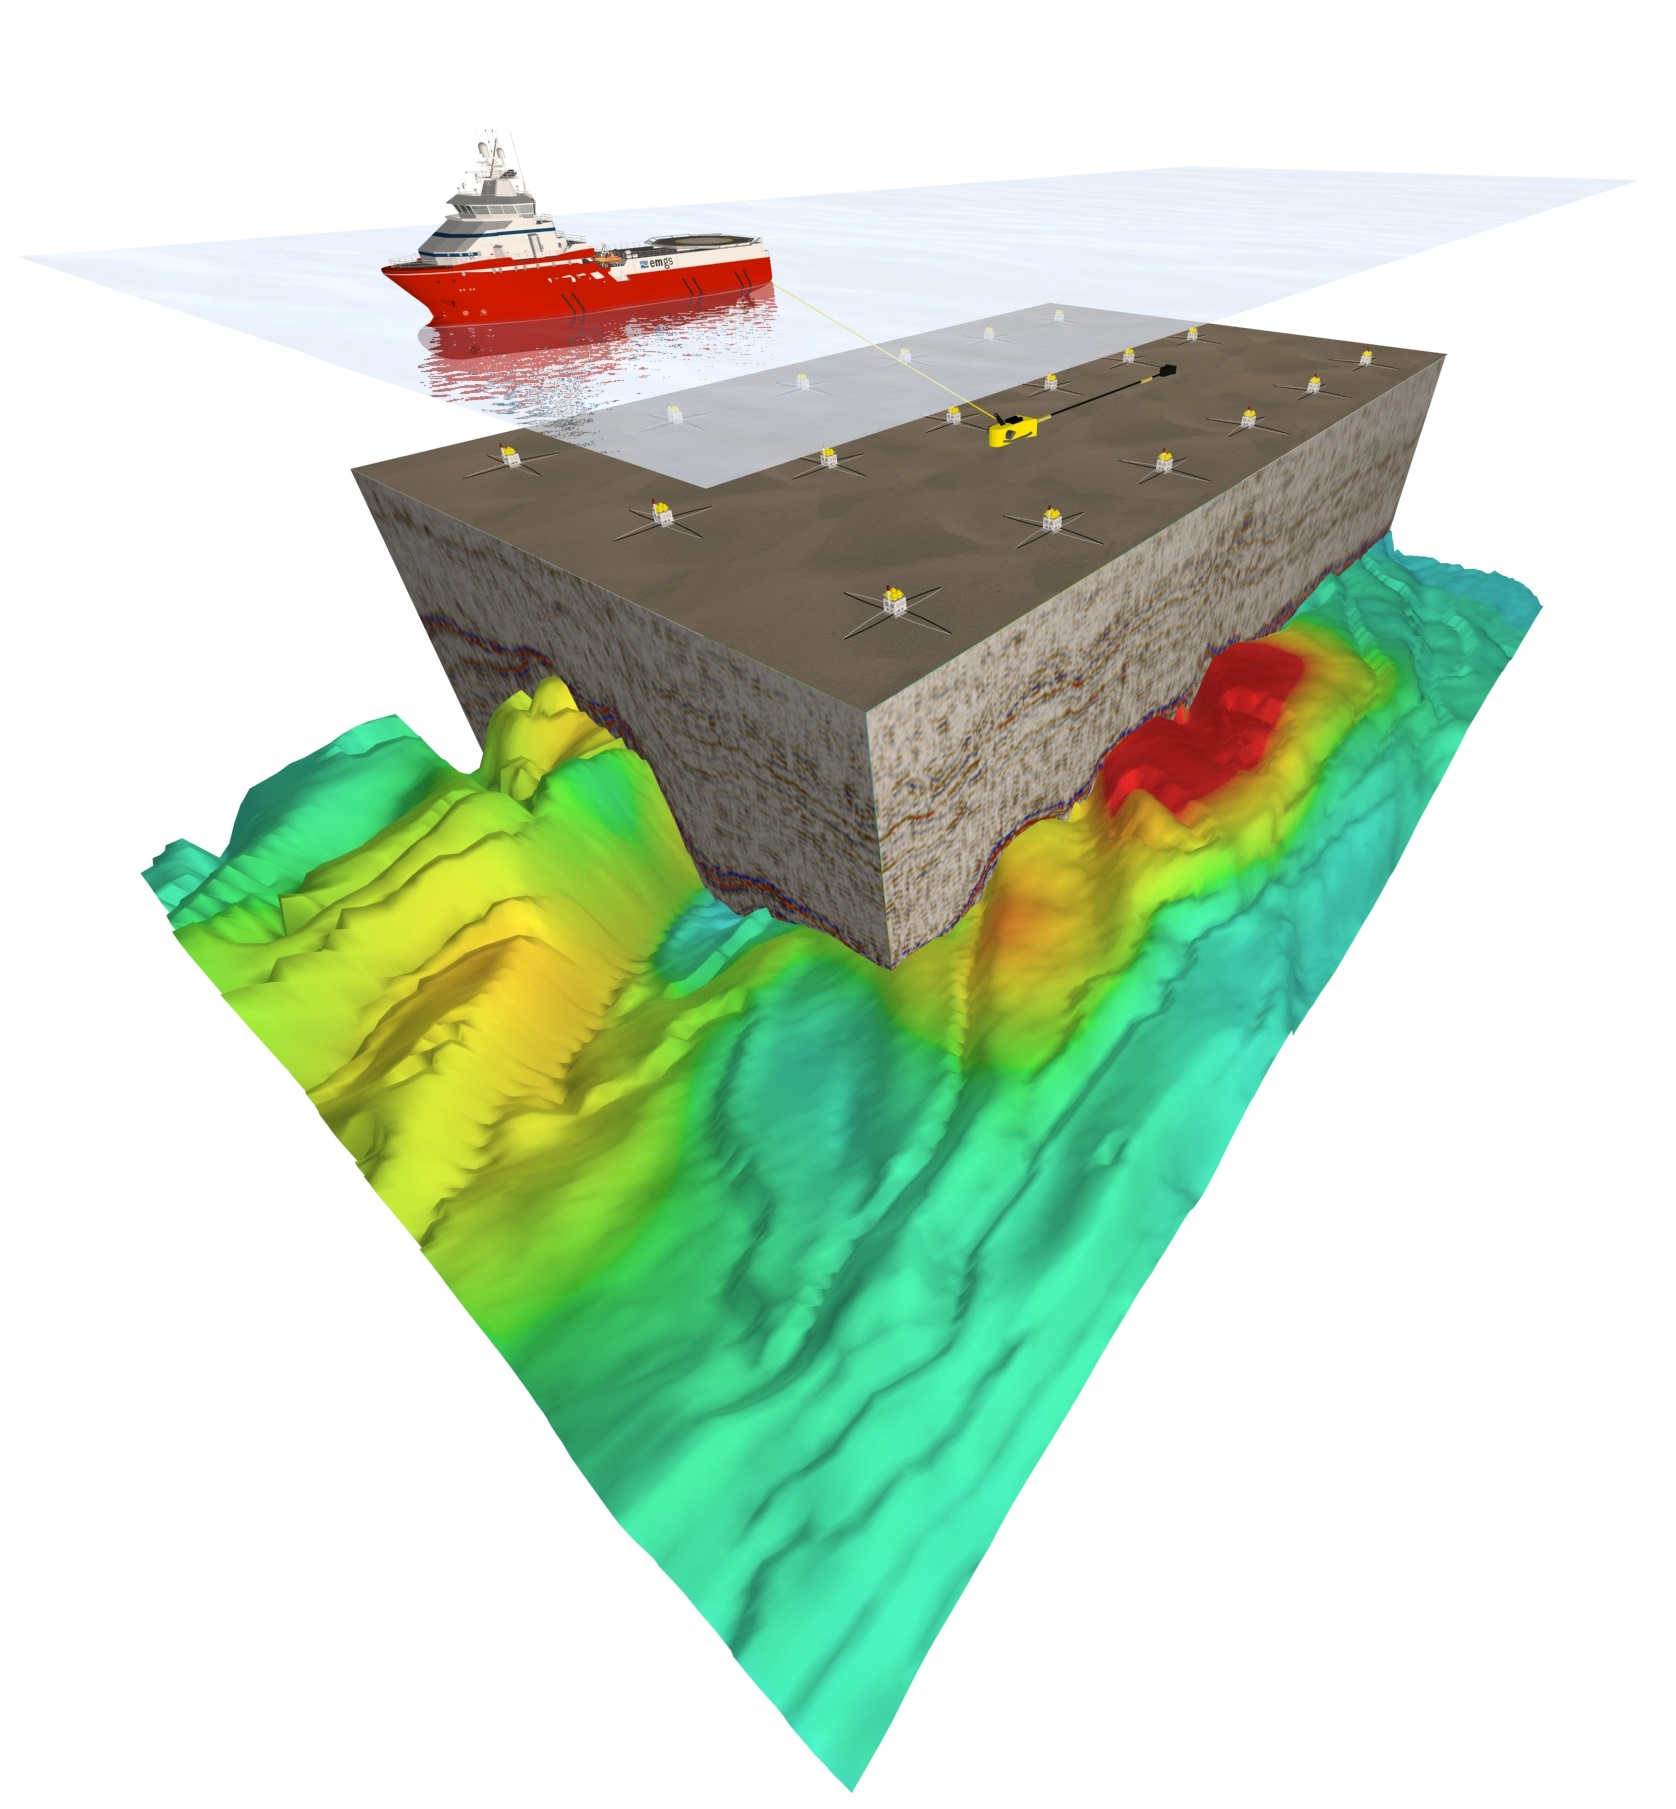
\includegraphics[width=3cm, trim=200 800 200 150, clip]{CSEM_Method3}};
        \node [color=white, xshift=1.5cm, yshift=1.4cm, rotate=60] (current page.south west) {\small \copyright\ emgs.com};
      \end{tikzpicture}
      %
      \centering
      \small \alert{Werthmüller, Rochlitz, Castillo-Reyes, and Heagy, 2020},\\
      submitted to GJI;
      \href{https://arxiv.org/abs/2010.12926}{arXiv:~2010.12926}
  \end{columns}
  %
  \note{
    \phantom{~}\\\hspace{1cm} \alert{\bfseries Summary Slide 1: Project Motivation}
    \begin{itemize}
      \item Large scale CSEM modelling with open-source software
      \item Opens new questions: validation; importance of mesh; repeatibility
    \end{itemize}
  }
\end{frame}

\begin{frame}[c]
  {Successful cross-validation between different codes and mesh types}
  %
  \begin{columns}[c]
    \column{.45\textwidth}
      \centering
      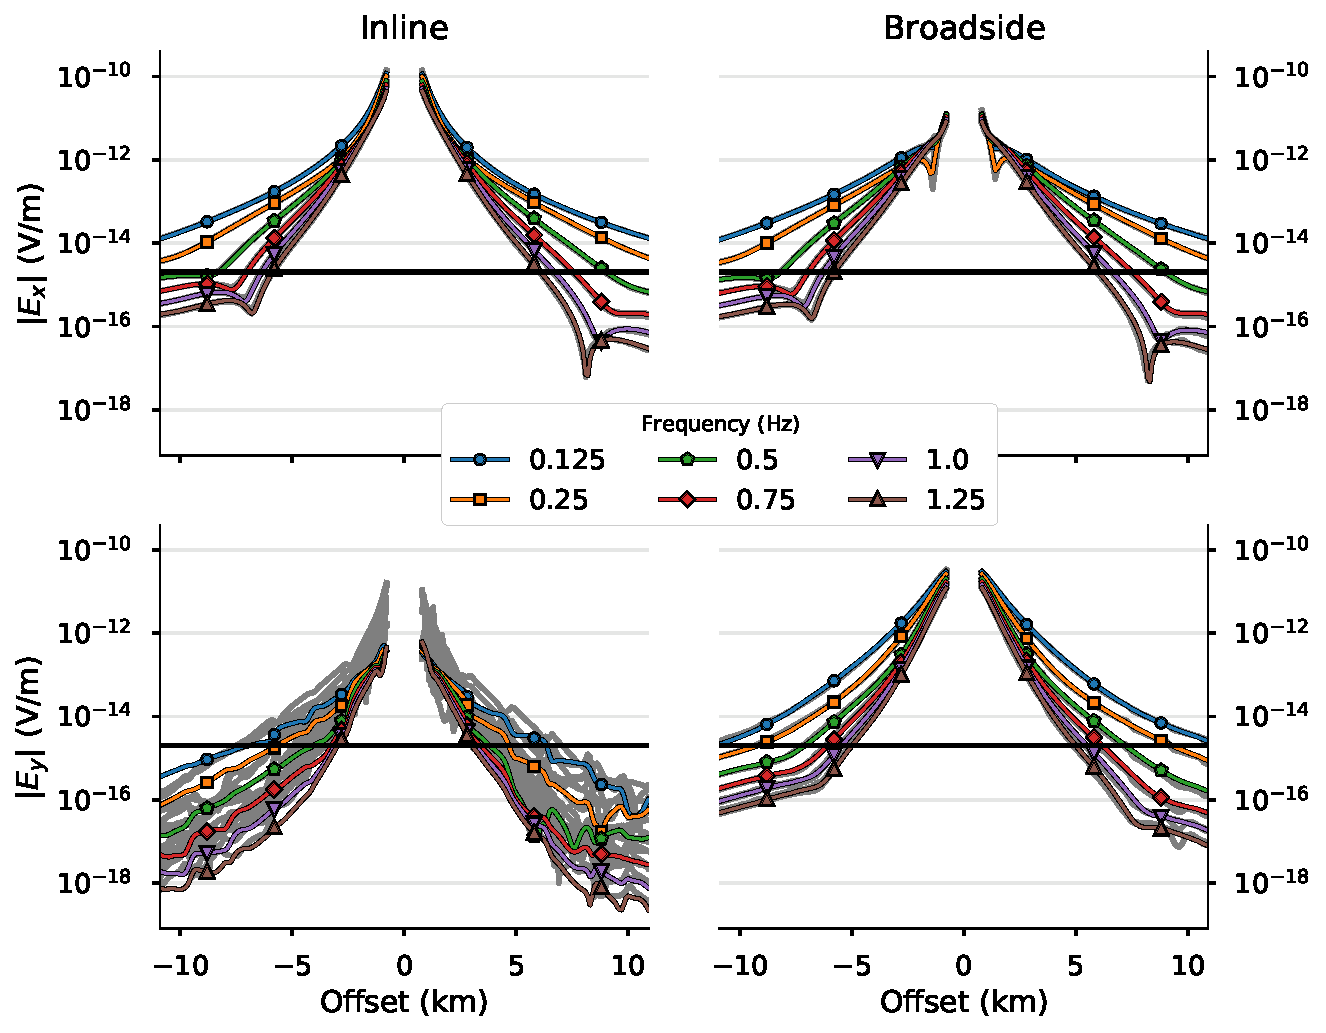
\includegraphics[width=\textwidth]{results-marlim-responses}
    \column{.55\textwidth}
      \centering
      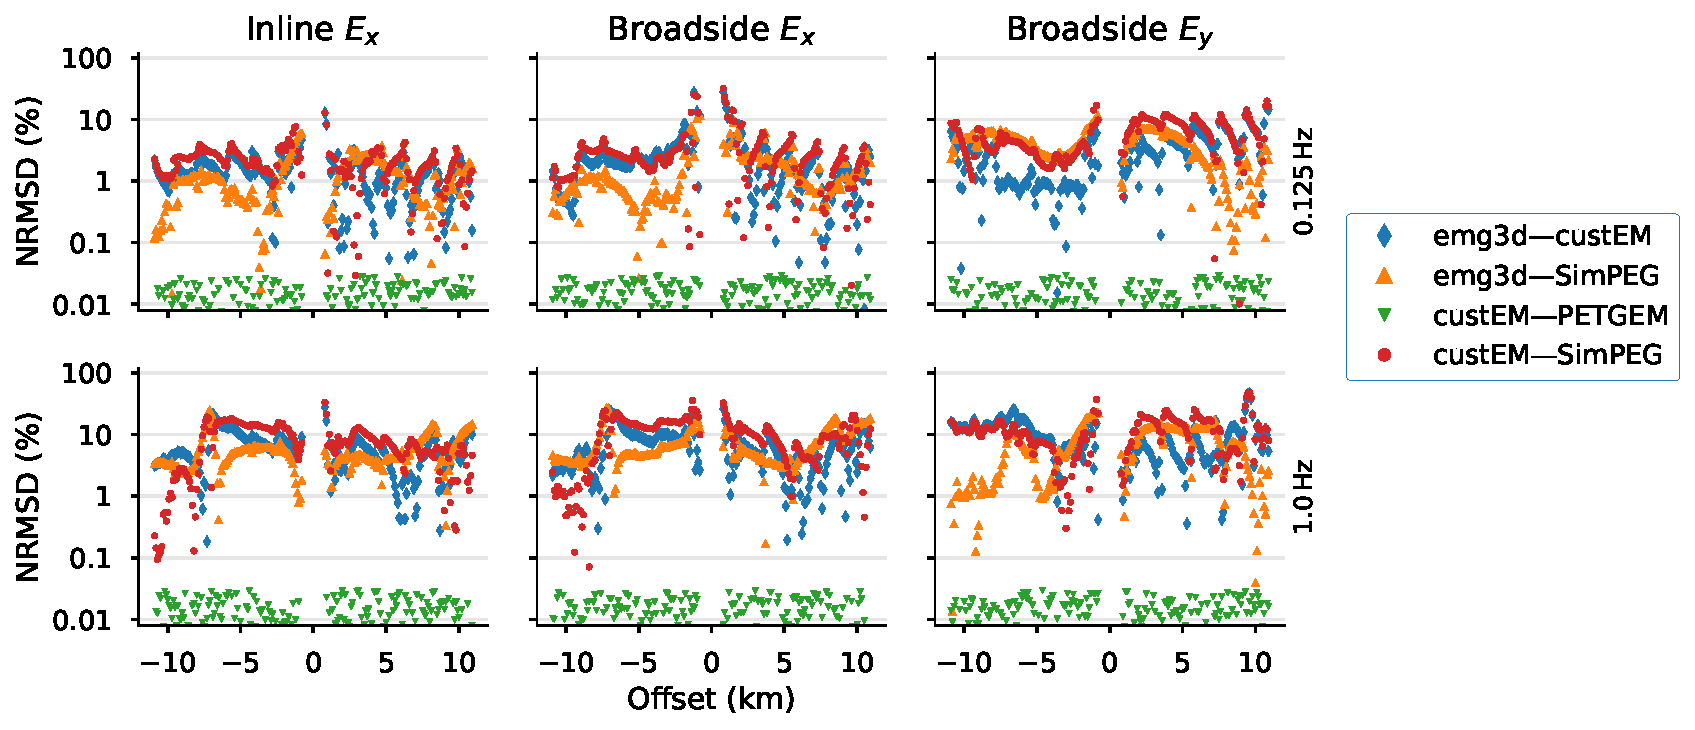
\includegraphics[width=\textwidth, trim=0 0 170 0, clip]{results-marlim_2ours}\\[.2cm]
      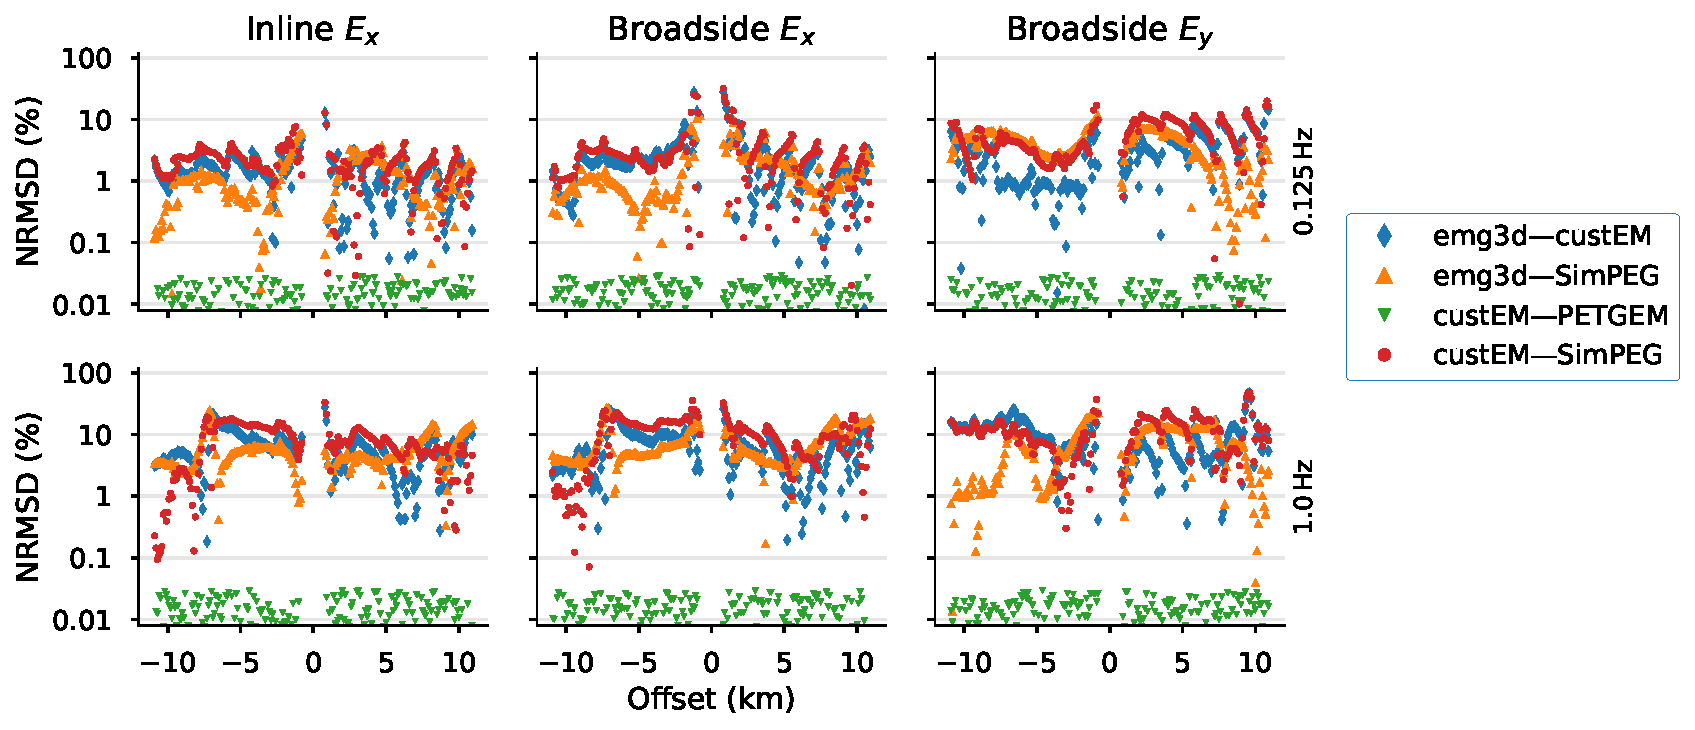
\includegraphics[width=.3\textwidth, trim=640 160 0 100, clip]{results-marlim_2ours}
  \end{columns}
  %
  \note{
    \phantom{~}\\\hspace{1cm} \alert{\bfseries Summary Slide 2: Key Results}
    \begin{itemize}
      \item Successfully modelled and validated different models
      \item Cross-validating 3D CSEM results with other codes is the\\
        only possible check
    \end{itemize}
  }
  %
\end{frame}

\begin{frame}
  {Comparisons, Validations, Benchmarks; Open-Source}
  \centering
  %
  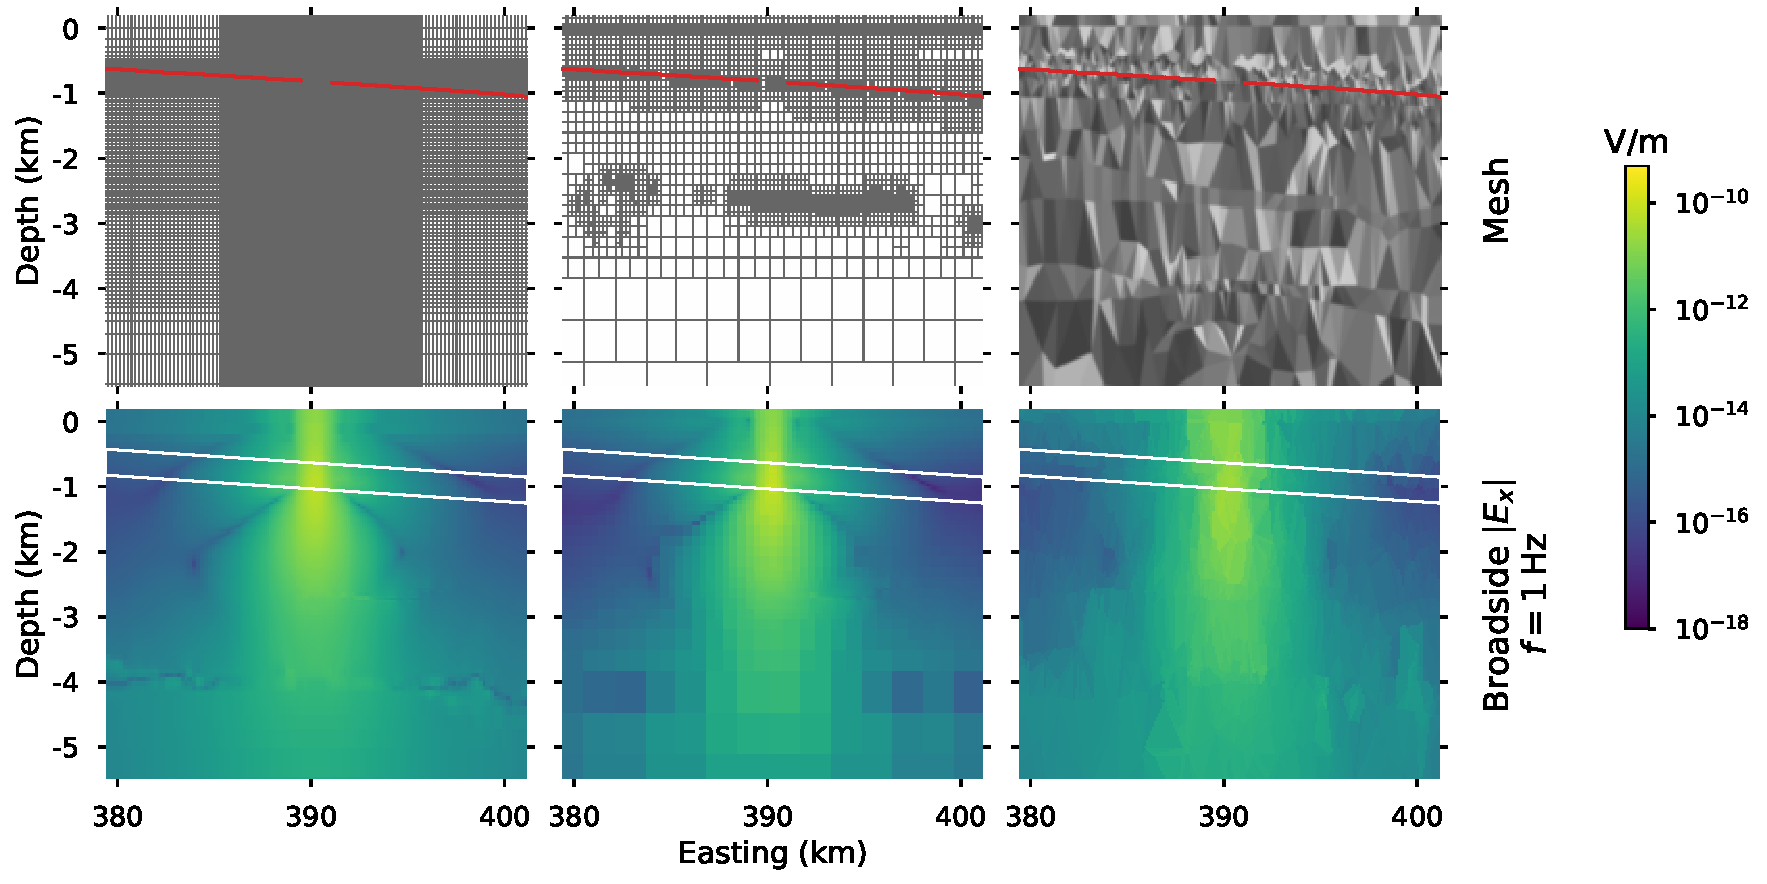
\includegraphics[width=.8\textwidth]{results-marlim_survey}\\[.5cm]
  %
  \href{mailto:d.werthmuller@tudelft.nl}{D.Werthmuller@TUDelft.nl}\\
  \alert{\bdra
    \href{https://github.com/swung-research/3d-csem-open-source-landscape}%
         {github.com/swung-research/3d-csem-open-source-landscape}
       \bdla}
  %
  \note{
    \phantom{~}\\\hspace{1cm} \alert{\bfseries Summary Slide 3: Significance}
    \begin{itemize}
      \item Comparisons, validations, and benchmarks are crucial for 3D
        modelling
      \item We need many more of them, which would benefit the community
      \item Other scenarios: air borne, topography, conductor, other sources
      \item Everything is on GitHub
    \end{itemize}
  }
  %
\end{frame}

\end{document}
